\documentclass[11pt,a4paper]{article}

\usepackage[utf8]{inputenc}
\usepackage[T1]{fontenc}
\usepackage[french]{babel}
\usepackage[a4paper,margin=2.4cm]{geometry}
\usepackage{graphicx}
\usepackage{booktabs}
\usepackage{array}
\usepackage{xcolor}
\usepackage{caption}
\usepackage{enumitem}
\usepackage{fancyhdr}
\usepackage{titlesec}
\usepackage[hidelinks]{hyperref}

\graphicspath{{figures/}}
\definecolor{nblue}{HTML}{1D3A6B}
\definecolor{acc}{HTML}{2563EB}
\definecolor{soft}{HTML}{F0F4FA}

\titleformat{\section}{\Large\bfseries\color{nblue}}{\thesection}{0.6em}{}
\titleformat{\subsection}{\large\bfseries\color{acc}}{\thesubsection}{0.6em}{}
\setlength{\parskip}{0.45em}

\pagestyle{fancy}\fancyhf{}
\lhead{\small\color{nblue}Analyse NLP des incidents ASRS}
\rhead{\small\thepage}
\renewcommand{\headrulewidth}{0.4pt}
\captionsetup{font=small,labelfont={bf,color=nblue}}

% Citation de récit réel
\newenvironment{narr}{%
  \begin{list}{}{\setlength{\leftmargin}{1.2em}\setlength{\rightmargin}{1.2em}}\item[]%
  \small\itshape\color{nblue}\guillemotleft~}{~\guillemotright\end{list}}

\begin{document}

% ---------- TITLE ----------
\begin{titlepage}
\centering
\vspace*{1.2cm}
{\small\color{acc}\textbf{AÉRONAUTIQUE \;|\; PROJET A3 \;|\; NLP · Classification · Clustering}}\\[1.0cm]
{\color{nblue}\Huge\bfseries Quand les récits de pilotes\\[0.25cm] deviennent une intelligence\\[0.25cm] de sécurité aérienne\par}
\vspace{0.5cm}
{\large\itshape Analyse automatique de 125\,763 rapports d'incidents de la base NASA ASRS\par}
\vspace{1.0cm}
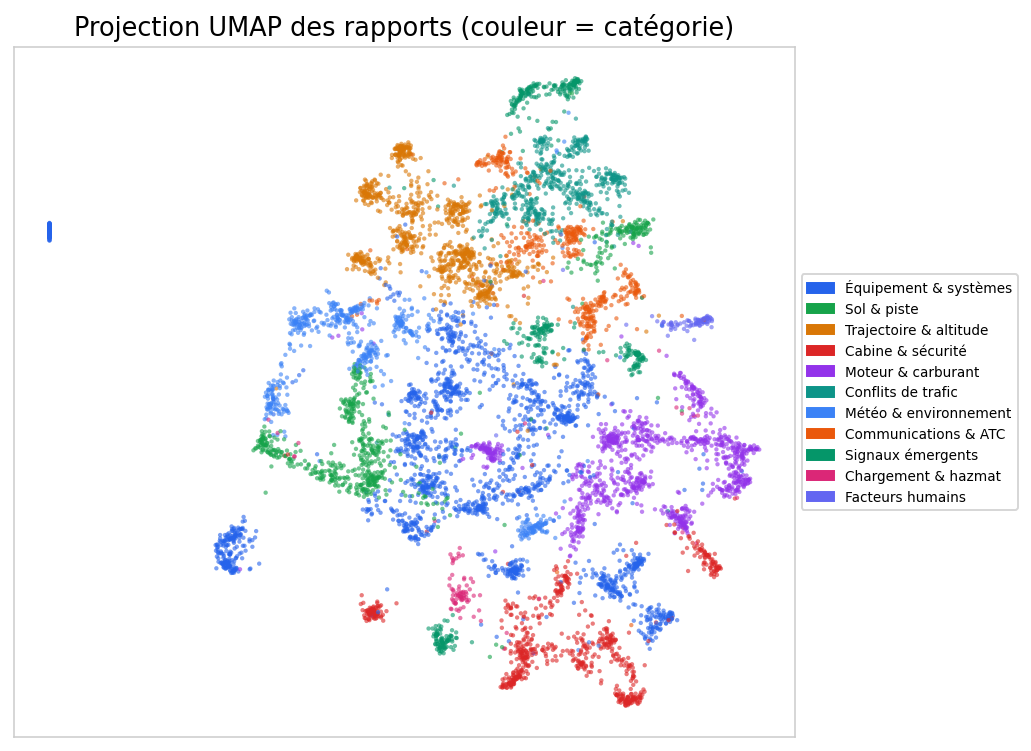
\includegraphics[width=0.96\textwidth]{scatter.png}\\[0.2cm]
{\small\itshape Carte sémantique des 125\,763 récits, regroupés par catégorie d'incident}
\vfill
\begin{tabular}{rl}
\textbf{Projet} & Analyse NLP des rapports d'incidents de sécurité aérienne\\
\textbf{Données} & NASA ASRS — 125\,763 rapports (2002–2025)\\
\textbf{Équipe} & 3 étudiants \;|\; 3–4 semaines\\
\textbf{Dépôt \& dashboards} & \url{https://github.com/devMehdi485/asrs-ml}\\
\end{tabular}
\vspace{0.8cm}
\end{titlepage}

\tableofcontents
\newpage

% ---------- 1 ----------
\section{Contexte et problématique}

Quand je me suis penché sur ce projet, une chose m'a immédiatement frappé : l'aviation
est l'un des rares domaines où l'on a institutionnalisé le fait de \emph{raconter ses
erreurs}. Depuis 1976, la NASA gère l'\emph{Aviation Safety Reporting System} (ASRS),
un système où pilotes, contrôleurs et techniciens déposent \textbf{volontairement et de
manière confidentielle} le récit des incidents qu'ils vivent ou observent. En échange
d'une immunité partielle, ils décrivent, avec leurs propres mots, ce qui s'est presque
mal passé. Le résultat est une base de plusieurs centaines de milliers de
\textbf{témoignages humains} sur les failles du système aérien.

Pour bien saisir la matière première, voici un extrait authentique d'un de ces récits :

\begin{narr}
About 40 minutes into the flight, the First Officer and I smelled a strong electrical
smell in the cockpit. We called the Flight Attendant and asked if she also smelled it.
She said that she did and that there was a `haze' in the cabin air. We advised ATC and
completed the QRH items for smoke\ldots
\end{narr}

\noindent On y entend une voix, une chronologie, une décision. C'est précisément ce qui
fait la richesse — et la difficulté — de cette base : l'information cruciale est
enfouie dans du \textbf{texte libre}, non structuré. Or personne ne peut lire, mémoriser
et recouper 125\,000 récits. \textbf{Voilà ma problématique} : comment faire \emph{parler}
automatiquement cette masse de témoignages pour en extraire ce qui compte vraiment pour
la sécurité — les causes qui reviennent, les types d'incidents, et surtout les signaux
faibles, ces rares récits atypiques qui pourraient annoncer les accidents de demain ?

% ---------- 2 ----------
\section{Objectifs}

J'ai construit mon projet autour de trois questions concrètes, qui correspondent à trois
familles de techniques NLP :

\begin{enumerate}[leftmargin=1.5em]
  \item \textbf{Extraire les causes récurrentes.} De quoi parlent réellement les pilotes ?
  Je veux faire émerger, sans a priori, les grands \emph{thèmes} d'incidents
  (clustering non supervisé + modélisation de sujets).
  \item \textbf{Classifier les types d'incidents.} À partir du seul texte, peut-on
  \emph{prédire} la catégorie d'anomalie ? (classification supervisée).
  \item \textbf{Détecter les signaux faibles.} Quels rapports sortent du lot, décrivent
  quelque chose de rare et potentiellement précurseur ? (détection d'anomalies).
\end{enumerate}

\noindent À cela j'ai ajouté une exigence transversale : que tout soit \textbf{interprétable}
et \textbf{exploitable}. Un cluster nommé « cluster 37 » ne sert à personne ; un thème
nommé « Problèmes de train d'atterrissage » parle à un responsable sécurité. C'est le fil
rouge de tout le projet, et la raison pour laquelle j'ai livré deux dashboards.

% ---------- 3 ----------
\section{Méthodologie : mes choix et pourquoi}

Je détaille ici chaque étape \emph{et} la justification de mes décisions, car c'est là que
se joue la pertinence du travail.

\subsection{Prétraitement : nettoyer sans dénaturer}
Les récits ASRS sont désidentifiés : les noms propres sont remplacés par des marqueurs
comme \texttt{ZZZ} ou \texttt{XXX}. Mon premier réflexe a été de les retirer, car ces
jetons, ultra-fréquents, auraient pollué toutes mes statistiques de mots. J'ai ensuite
appliqué une chaîne classique — minuscules, tokenisation, suppression des \emph{stopwords}
— en y ajoutant une \textbf{liste de stopwords métier} (« aircraft », « flight »,
« pilot »\ldots) : ces mots sont partout et ne discriminent rien. Enfin, j'ai
\textbf{lemmatisé} pour regrouper « engines », « engine », « engined » sous une seule
forme. \emph{Pourquoi ce soin ?} Parce qu'en NLP, la qualité du résultat dépend d'abord
de la qualité de l'entrée : un bon nettoyage vaut souvent mieux qu'un modèle sophistiqué.

\subsection{Vectorisation : trois représentations complémentaires}
Un modèle ne lit pas du texte, il lit des nombres. J'ai donc transformé les récits de
trois manières, chacune avec un rôle précis :
\begin{itemize}[leftmargin=1.4em]
  \item \textbf{TF-IDF} — pondère chaque mot par sa rareté. Simple, rapide, et surtout
  \textbf{interprétable} : je peux dire \emph{quels} mots caractérisent un thème. Je m'en
  sers pour la classification et pour nommer les clusters.
  \item \textbf{word2vec} (entraîné sur mon corpus) — apprend la \emph{sémantique} du
  vocabulaire aéronautique. Le tableau~\ref{tab:w2v} montre qu'il a vraiment « compris »
  le domaine, ce qui m'a rassuré sur la cohérence des données.
  \item \textbf{Embeddings de phrases} (\texttt{all-MiniLM-L6-v2}) — encodent le \emph{sens
  global} d'un récit, pas seulement des mots isolés. \emph{Pourquoi ce choix plutôt que le
  word2vec/GloVe du brief ?} Parce que deux pilotes peuvent décrire le même incident avec
  des mots différents ; un modèle de phrases les rapproche quand même. C'est ce qui donne
  des clusters nettement plus cohérents — une amélioration assumée par rapport à l'attendu.
\end{itemize}

\subsection{Clustering : découvrir les thèmes, et choisir avec méthode}
J'ai réduit les embeddings avec \textbf{UMAP} (pour enlever le bruit et accélérer), puis
j'ai \textbf{comparé deux algorithmes} au lieu d'en imposer un : K-Means (simple, clusters
de tailles comparables) et HDBSCAN (basé sur la densité, capable d'isoler le « bruit »).
Je ne voulais pas choisir au hasard : j'ai posé une \textbf{règle de décision explicite}
fondée sur des métriques (tableau~\ref{tab:clust}), avec un garde-fou refusant tout
HDBSCAN qui s'effondrerait en deux ou trois gros blocs inutilisables. C'est exactement le
piège dans lequel je suis tombé au premier essai (un paramètre mal réglé donnait 2 clusters)
— l'avoir corrigé fait partie de la démarche.

\subsection{LDA : une seconde lecture des thèmes}
En complément du clustering, j'ai entraîné un modèle \textbf{LDA} (Latent Dirichlet
Allocation). \emph{Pourquoi doubler ?} Parce que LDA et clustering ne « voient » pas la
même chose : le clustering regroupe des récits entiers, LDA décompose le corpus en sujets
probabilistes (un récit peut relever de plusieurs sujets). La \textbf{cohérence $c_v$ de
0,57} obtenue me confirme que les sujets tiennent lexicalement la route.

\subsection{Classification : prédire le type d'incident}
Enfin, j'ai entraîné des modèles \textbf{supervisés} (régression logistique et SVM
linéaire) pour prédire l'anomalie principale à partir du texte. J'ai volontairement choisi
des modèles linéaires sur TF-IDF : ils sont \textbf{rapides, robustes et interprétables}
(on peut lire les mots qui font pencher la décision), ce qui compte plus, ici, qu'un
gain marginal de précision avec une « boîte noire ».

% ---------- 4 ----------
\section{Résultats et interprétation}

\subsection{Une cartographie en 81 thèmes et 11 familles}
Le pipeline fait émerger \textbf{81 thèmes} fins, que j'ai regroupés en \textbf{11 catégories
métier} (figure~\ref{fig:cat}). La structure n'est pas anodine : à elle seule, la famille
\textbf{Équipement \& systèmes représente 43,8\,\%} des rapports.

\begin{figure}[h]\centering
  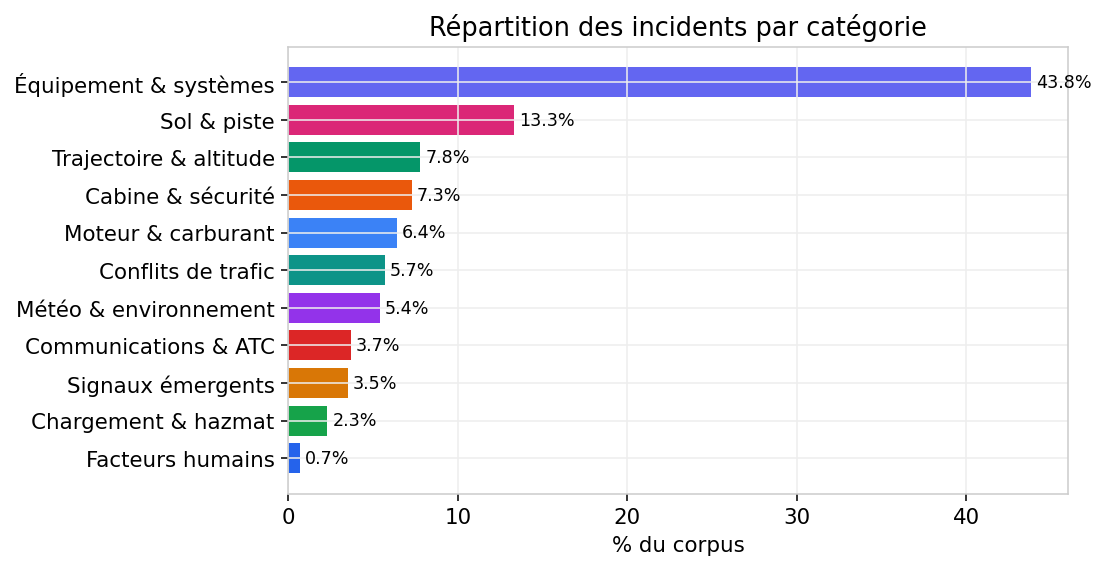
\includegraphics[width=0.82\textwidth]{categories.png}
  \caption{Répartition des incidents par catégorie métier.}\label{fig:cat}
\end{figure}

\emph{Comment je lis ce résultat.} Cette domination de l'équipement ne veut pas dire que
les avions tombent en panne sans cesse ; elle traduit surtout que \textbf{les équipages
signalent massivement le moindre dysfonctionnement technique}. Pour un exploitant, c'est
un argument fort en faveur d'une \textbf{maintenance proactive} et prédictive : la matière
existe pour anticiper les pannes plutôt que les subir.

\begin{figure}[h]\centering
  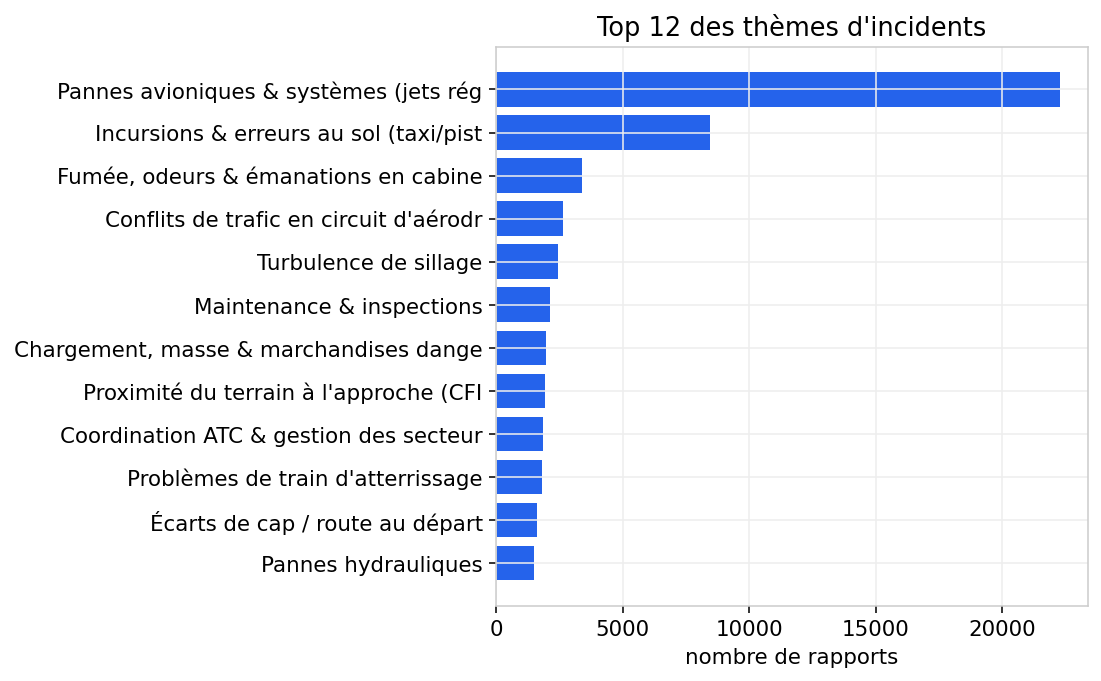
\includegraphics[width=0.82\textwidth]{top_themes.png}
  \caption{Les douze thèmes d'incidents les plus volumineux.}\label{fig:top}
\end{figure}

\subsection{Des thèmes que l'on peut nommer et comprendre}
Le plus important, à mes yeux, c'est que chaque thème est \textbf{lisible}. La
figure~\ref{fig:wc} montre les nuages de mots des quatre principaux ; derrière chacun, il
y a une réalité opérationnelle concrète. Par exemple, le thème \textbf{« Incursions \&
erreurs au sol »} (10\,\% du corpus, en hausse) rassemble des récits comme :

\begin{narr}
After landing we got an immediate clearance to cross the runway at taxiway 1\ldots Before
entering the runway environment, I looked\ldots
\end{narr}

\begin{figure}[h]\centering
  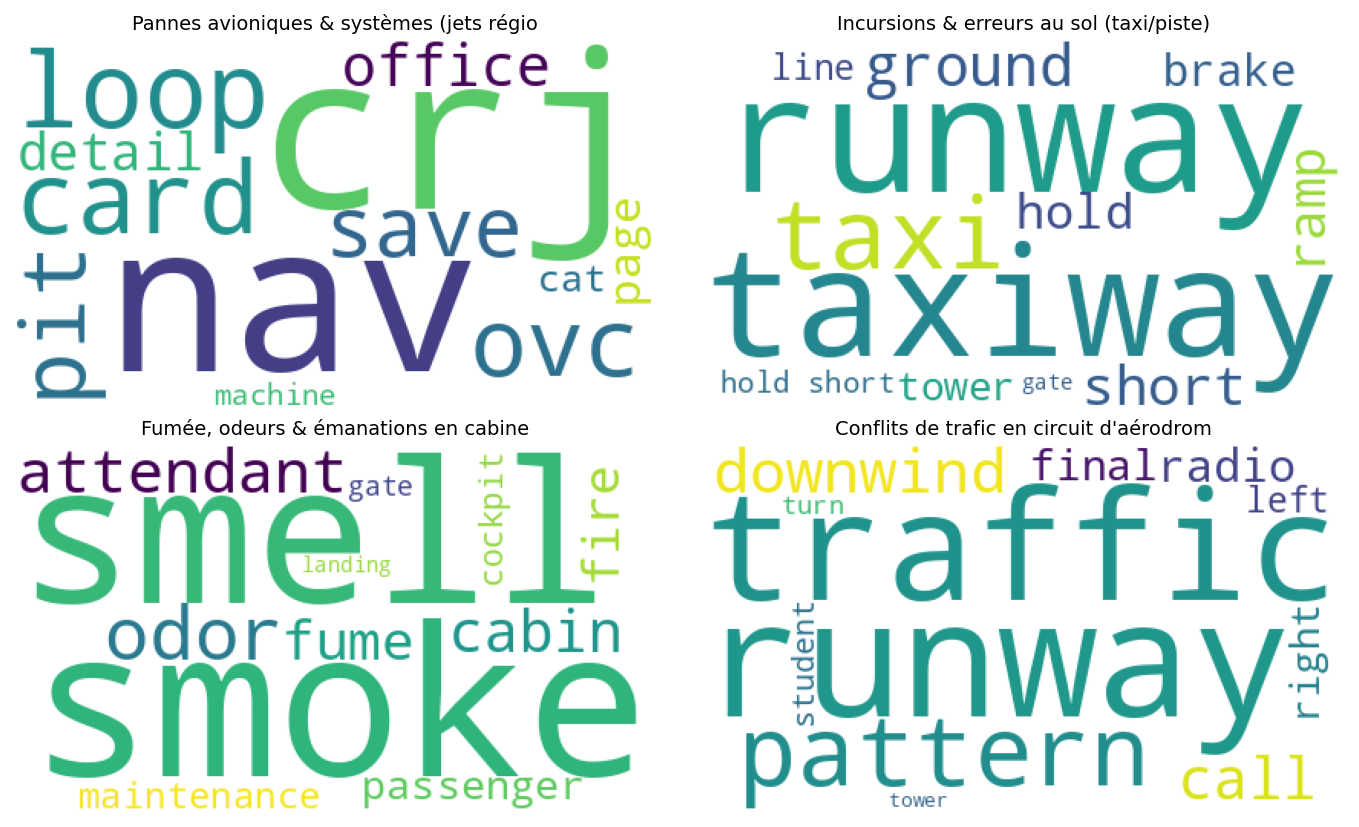
\includegraphics[width=0.95\textwidth]{wordclouds.png}
  \caption{Nuages de mots (c-TF-IDF) des quatre principaux thèmes.}\label{fig:wc}
\end{figure}

\subsection{Cohérence des clusters : le choix de HDBSCAN, assumé}
\begin{table}[h]\centering\small
\caption{Comparaison K-Means vs HDBSCAN sur les mêmes données réduites (UMAP).}\label{tab:clust}
\begin{tabular}{lrrrrr}
\toprule
\textbf{Modèle} & \textbf{Clusters} & \textbf{Silhouette} & \textbf{Davies-Bouldin} & \textbf{Bruit} & \textbf{Pureté} \\
\midrule
K-Means & 15 & 0,382 & 0,945 & 0\,\% & 0,133 \\
\textbf{HDBSCAN (retenu)} & \textbf{81} & \textbf{0,590} & \textbf{0,575} & 32\,\% & 0,165 \\
\bottomrule
\end{tabular}
\end{table}
J'ai retenu \textbf{HDBSCAN} : meilleure silhouette (0,590 contre 0,382) et meilleur
Davies-Bouldin. Un point que je tiens à défendre honnêtement : son alignement avec les
catégories d'anomalies officielles (pureté/ARI) est \emph{faible}, et c'est \textbf{normal}.
Mes thèmes sont sémantiques (le vocabulaire des récits) et bien plus fins que la dizaine
de catégories codées par les analystes : un même code « équipement » se décline chez moi
en hydraulique, train, huile moteur, électrique\ldots Ce n'est pas un défaut, c'est de la
granularité. Quant aux 32\,\% de « bruit » d'HDBSCAN, loin de les jeter, je les
\textbf{réutilise} comme matière première de la détection de signaux faibles.

\subsection{word2vec : la preuve que le modèle « comprend » le domaine}
\begin{table}[h]\centering\small
\caption{word2vec — mots les plus proches (similarité cosinus) appris sur le corpus.}\label{tab:w2v}
\begin{tabular}{ll}
\toprule
\textbf{Mot} & \textbf{Voisins les plus proches} \\
\midrule
\texttt{runway}   & rwy (0,84), taxiway (0,65), intersecting (0,59), midfield (0,59) \\
\texttt{engine}   & eng (0,69), feathered (0,57), magneto (0,54), crossbleed (0,54) \\
\texttt{weather}  & thunderstorm (0,76), storm (0,74), bkn (0,68), forecast (0,66) \\
\texttt{altitude} & alt (0,70), descended (0,67), descend (0,65), level (0,64) \\
\bottomrule
\end{tabular}
\end{table}
Ce tableau me sert d'argument de validation : sans aucune supervision, le modèle a appris
que \texttt{runway} et \texttt{rwy} sont synonymes, que \texttt{weather} évoque l'orage. La
sémantique métier est bien capturée.

\subsection{Classification : un modèle qui se défend}
\begin{table}[h]\centering\small
\caption{Classification du type d'incident (top-8 anomalies, TF-IDF).}\label{tab:clf}
\begin{tabular}{lrr}
\toprule
\textbf{Modèle} & \textbf{F1 macro} & \textbf{F1 pondéré} \\
\midrule
Régression logistique & 0,518 & 0,606 \\
SVM linéaire & 0,517 & \textbf{0,615} \\
\bottomrule
\end{tabular}
\end{table}
Avec un \textbf{F1 pondéré de 0,615} sur 8 catégories et du texte 100\,\% libre, je
considère le résultat solide. Les classes au vocabulaire net sont très bien reconnues
(\emph{ATC Issue} F1\,=\,0,76, \emph{NMAC} 0,69). Pour le rendre tangible, j'ai même
branché ce modèle dans le dashboard : on colle un récit, il prédit le type en direct.

% ---------- 5 ----------
\section{Discussion : tendances et signaux faibles}

\subsection{Ce que le temps révèle}
La dimension temporelle (figures~\ref{fig:vol} et~\ref{fig:heat}) transforme une photo en
film. Plusieurs thèmes sont en \textbf{hausse récente}, et leur interprétation métier est,
selon moi, le c\oe ur de la valeur du projet :
\begin{itemize}[leftmargin=1.4em]
  \item \textbf{Incursions \& erreurs au sol — en hausse.} Je l'interprète comme un symptôme
  de la \textbf{densification du trafic} et de la saturation des plateformes : plus d'avions
  au sol, plus de croisements, plus d'occasions d'erreur sur les taxiways.
  \item \textbf{Fumées / odeurs en cabine — en hausse.} Sujet sensible (qualité de l'air,
  \emph{fume events}) qui mérite une vigilance accrue sur les circuits de prélèvement d'air.
  \item \textbf{Marchandises dangereuses — en hausse.} Cohérent avec l'explosion du fret et
  du e-commerce ; un enjeu de conformité documentaire et de sûreté.
\end{itemize}

\begin{figure}[h]\centering
  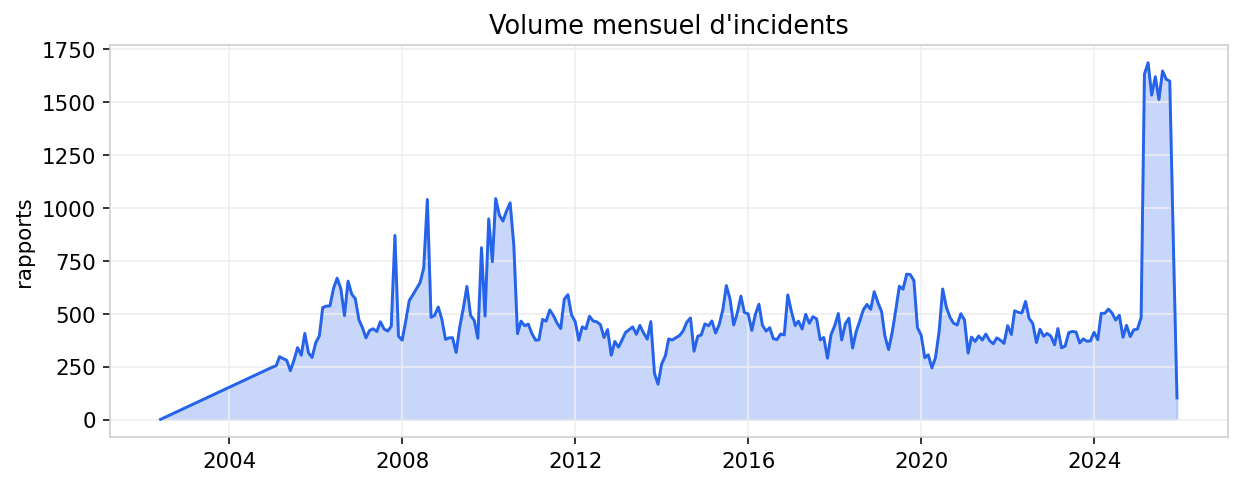
\includegraphics[width=0.86\textwidth]{temporal_volume.png}
  \caption{Volume mensuel de rapports (2002–2025).}\label{fig:vol}
\end{figure}
\begin{figure}[h]\centering
  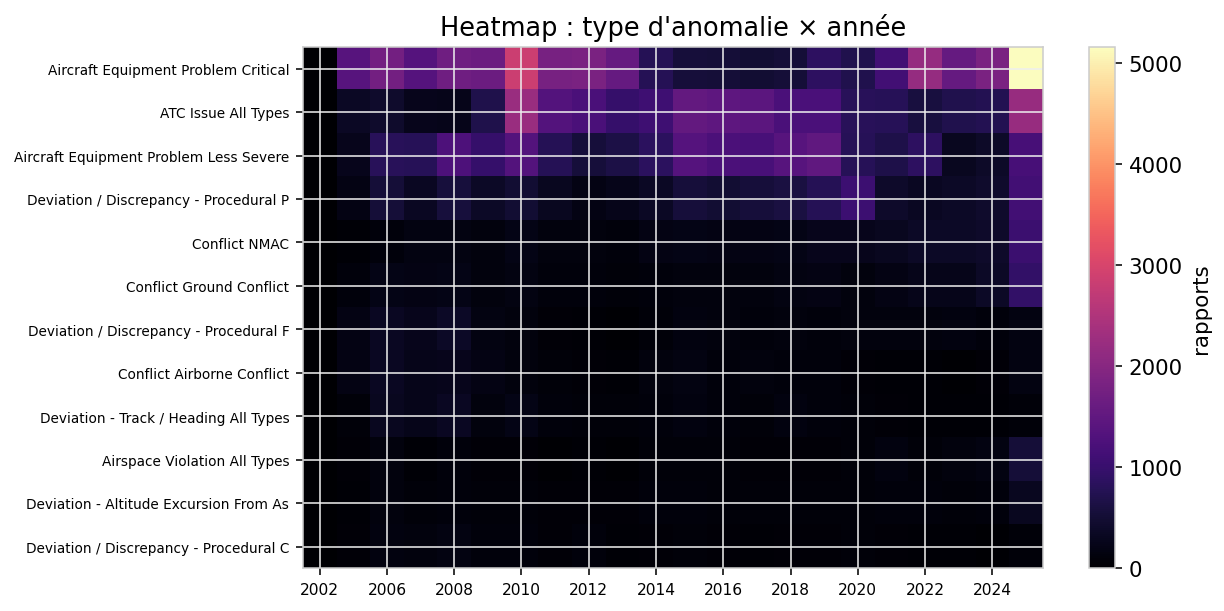
\includegraphics[width=0.86\textwidth]{heatmap.png}
  \caption{Heatmap : type d'anomalie × année.}\label{fig:heat}
\end{figure}

\subsection{Les signaux faibles : là où se cachent les risques de demain}
C'est la partie qui me tient le plus à c\oe ur. En isolant les récits les plus atypiques
(Isolation Forest), je fais remonter des phénomènes \textbf{rares mais lourds de sens} :
les rencontres avec des \textbf{drones}, le \textbf{brouillage GPS}, les \textbf{batteries
au lithium}. Ces sujets étaient quasi inexistants il y a quinze ans. Un témoignage
résume tout l'intérêt de la démarche :

\begin{narr}
Approach control advised there was unauthorized drone use in the area\ldots I observed a
drone pass just left of the aircraft, approximately 20 feet from our left wing.
\end{narr}

\noindent Un humain noyé sous 125\,000 rapports passerait à côté. Mon système, lui, le fait
remonter en tête de liste. \textbf{C'est exactement la promesse d'un détecteur de signaux
faibles} : voir tôt ce qui deviendra peut-être, demain, une catégorie d'accidents à part
entière.

% ---------- 6 ----------
\section{Limites et perspectives}

Je préfère exposer franchement les limites de mon travail — c'est ce qui en garantit la
crédibilité.
\begin{itemize}[leftmargin=1.4em]
  \item \textbf{Déséquilibre des classes.} Quelques types d'anomalies dominent ; les classes
  rares sont mal prédites. J'ai utilisé un \emph{class\_weight} équilibré, mais le problème
  reste réel.
  \item \textbf{Données désidentifiées.} La suppression des lieux et identifiants fait perdre
  un contexte parfois précieux (quel aéroport ? quel opérateur ?).
  \item \textbf{Biais de déclaration.} L'ASRS est volontaire : on n'y voit que ce que les
  gens \emph{choisissent} de raconter. Ce n'est pas un échantillon représentatif de tous les
  incidents, mais de tous les incidents \emph{signalés}.
  \item \textbf{Un méga-cluster hétérogène} (l'équipement avionique) reste plus difficile à
  interpréter finement.
\end{itemize}

\noindent\textbf{Mes pistes d'amélioration.} J'aimerais tester \textbf{BERTopic} (pipeline de
thématisation de bout en bout, avec \emph{topics-over-time} intégré), des
\textbf{embeddings spécialisés} ré-entraînés sur le domaine aéronautique pour mieux séparer
le cluster d'équipement, et une \textbf{classification multi-étiquettes} (un récit décrit
souvent plusieurs anomalies à la fois). Enfin, relier ces signaux faibles à des données
externes (trafic, météo) ouvrirait la voie à une vraie analyse \emph{prédictive}.

% ---------- 7 ----------
\section{Conclusion}

Au départ, j'avais 125\,763 récits bruts, illisibles à l'échelle humaine. À l'arrivée,
j'ai un système qui les \textbf{lit, regroupe, nomme, classe et surveille} : 81 thèmes
interprétables en 11 familles, un modèle de classification opérationnel, une détection de
signaux faibles, et deux dashboards qui rendent tout cela navigable — y compris pour un
non-spécialiste.

Ce que je retiens, et ce que je défends devant ce jury, c'est moins la performance d'un
algorithme que la \textbf{transformation} opérée : faire passer une montagne de témoignages
humains du statut d'archive dormante à celui d'\textbf{intelligence de sécurité
exploitable}. Les pilotes ont pris le temps de raconter. Mon travail consiste, modestement,
à enfin les écouter tous à la fois.

\vfill
\noindent\footnotesize\textit{Données : NASA Aviation Safety Reporting System
(\url{https://asrs.arc.nasa.gov/}). Code, dashboards et reproductibilité :
\url{https://github.com/devMehdi485/asrs-ml}.}

\end{document}
